\chapter{Special Relativity}\index{special relativity}\index{relativity, special}

Your phone's GPS works by timing radio signals from satellites. The satellites carry atomic
clocks accurate to a billionth of a second. Yet engineers have to set those clocks to tick at
the wrong rate before launch, because once in orbit they run fast, by 38 millionths of a second
every day. Without that correction, your map would drift by about 11 kilometers a day.

Why would a perfect clock run fast in orbit? Because time itself does not pass at the same rate
for everyone. Moving clocks run slow. This was Albert Einstein's discovery in 1905, and it
sounds like science fiction. But you can derive it yourself in half a page, using nothing but
the Pythagorean theorem.

\section{A Puzzle About Light}
In the Electromagnetic Waves chapter, you saw that Maxwell's equations predict the speed of
light: $c = \frac{1}{\sqrt{\mu_0\epsilon_0}} \approx 3.00 \times 10^8$ m/s. That raised a strange
question: 300 million meters per second \emph{relative to what}? If you throw a ball forward at
20 m/s from a train moving at 30 m/s, the ball moves at 50 m/s relative to the ground. You would
expect light from a moving flashlight to work the same way. But Maxwell's formula contains no
speed of the source or the observer, just two constants of nature.

Experiments agreed with Maxwell. Light from the front and the back of the moving Earth, and from
fast-moving stars, always arrived at the same speed. Einstein took the result seriously and built
a new physics on two principles, called \newterm{postulates}:
\begin{enumerate}
\item \textbf{The laws of physics are the same for everyone moving at a steady velocity.} No
experiment inside a smoothly moving train, with the windows covered, can tell you how fast the
train is going.
\item \textbf{Everyone measures the same speed of light, $c$}, no matter how fast they or the
source are moving.
\end{enumerate}
Each sounds reasonable. Together, they force time to stretch.

\section{The Light Clock}\index{light clock}\index{time dilation}
Imagine the simplest possible clock: a pulse of light bouncing between two mirrors a distance $L$
apart. Each round trip is one ``tick.'' For someone holding the clock, the light travels $2L$ at
speed $c$, so one tick takes
$$\Delta t_0 = \frac{2L}{c}$$

\begin{figure}[H]
\centering
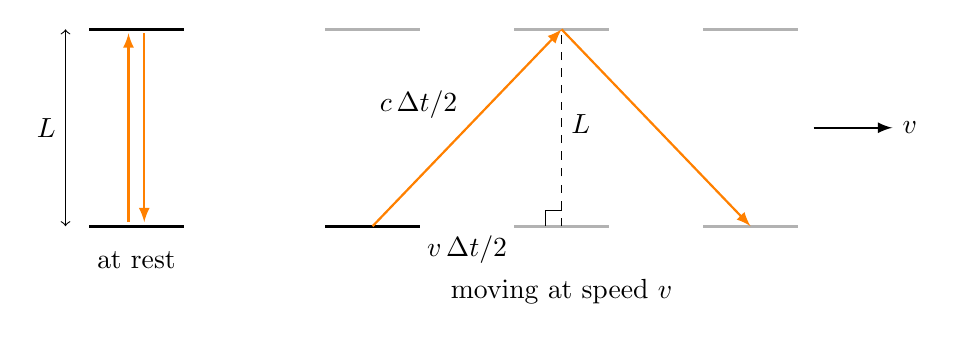
\begin{tikzpicture}[scale=1.0]
% clock at rest
\draw[very thick] (-0.6,0) -- (0.6,0);
\draw[very thick] (-0.6,2.5) -- (0.6,2.5);
\draw[-latex, thick, orange] (-0.1,0.05) -- (-0.1,2.45);
\draw[-latex, thick, orange] (0.1,2.45) -- (0.1,0.05);
\draw[<->] (-0.9,0) -- (-0.9,2.5) node[midway, left] {$L$};
\node[below] at (0,-0.2) {at rest};
% moving clock
\begin{scope}[xshift=3cm]
\foreach \x in {0,2.4,4.8} {
  \draw[very thick, gray!60] (\x-0.6,0) -- (\x+0.6,0);
  \draw[very thick, gray!60] (\x-0.6,2.5) -- (\x+0.6,2.5);
}
\draw[very thick] (-0.6,0) -- (0.6,0);
\draw[-latex, thick, orange] (0,0) -- (2.4,2.5);
\draw[-latex, thick, orange] (2.4,2.5) -- (4.8,0);
\draw[dashed] (2.4,0) -- (2.4,2.5);
\draw (2.2,0) -- (2.2,0.2) -- (2.4,0.2);
\node[below] at (1.2,0) {$v\,\Delta t/2$};
\node[right] at (2.4,1.3) {$L$};
\node[above left] at (1.2,1.25) {$c\,\Delta t/2$};
\draw[-latex, thick] (5.6,1.25) -- (6.6,1.25) node[right] {$v$};
\node[below] at (2.4,-0.55) {moving at speed $v$};
\end{scope}
\end{tikzpicture}
\caption{A light clock. Left: for someone holding it, the light bounces straight up and down.
Right: watched from the ground as the clock moves, the light travels a longer, slanted path.}
\label{fig:light-clock}
\end{figure}

Now put the clock on a spaceship moving past you at speed $v$. From the ground, the mirrors move
sideways while the light is in flight, so the light travels along a slanted path (figure
\ref{fig:light-clock}). The slanted path is longer. But by the second postulate, the light still
moves at exactly $c$. A longer path at the same speed takes more time.

Let $\Delta t$ be the time of one tick as measured from the ground. During half a tick, the light
travels $c\frac{\Delta t}{2}$ along the slant, while the clock moves $v\frac{\Delta t}{2}$ sideways.
Together with the height $L$, these form a right triangle, and the Pythagorean theorem gives
$$\left(\frac{c\Delta t}{2}\right)^2 = \left(\frac{v\Delta t}{2}\right)^2 + L^2$$
Solve for $\Delta t$:
$$\frac{\Delta t^2}{4}\left(c^2 - v^2\right) = L^2 \quad\Longrightarrow\quad
\Delta t = \frac{2L}{\sqrt{c^2 - v^2}} = \frac{2L/c}{\sqrt{1 - v^2/c^2}}$$
Since $\frac{2L}{c} = \Delta t_0$, this is

\begin{mdframed}[style = important, frametitle = {Time Dilation}]
$$\Delta t = \gamma\,\Delta t_0, \qquad \text{where } \gamma = \frac{1}{\sqrt{1 - v^2/c^2}}$$
Here $\Delta t_0$ is the time between two events measured by a clock that is present at both (the
\newterm{proper time}), and $\Delta t$ is the time measured by someone watching that clock move past at
speed $v$.
\end{mdframed}

The \newterm{Lorentz factor} $\gamma$ (the Greek letter gamma) is always at least 1, so moving clocks
run slow. Nothing about the argument depends on light clocks in particular. By the first postulate,
every clock on the ship, including the astronauts' heartbeats, must keep pace with the light clock.
Otherwise the astronauts could tell they were moving. \emph{Time itself} runs slow on the ship.

Here is $\gamma$ for a range of speeds:
\begin{center}
\begin{tabular}{l|c|l}
Speed & $v/c$ & $\gamma$ \\
\hline
A car on the highway (30 m/s) & $10^{-7}$ & $1.000000000000005$ \\
The International Space Station (7.7 km/s) & $2.6 \times 10^{-5}$ & $1.0000000003$ \\
Fast spaceship & 0.5 & 1.155 \\
Faster spaceship & 0.9 & 2.294 \\
Cosmic-ray muon & 0.995 & 10.0 \\
Particle in an accelerator & 0.999 & 22.4 \\
\end{tabular}
\end{center}
At everyday speeds, $\gamma$ is so close to 1 that nobody noticed relativity for all of human
history. Near the speed of light, it is dramatic.

\section{The Evidence: Muons}\index{muon}
Time dilation is not a thought experiment; it is measured every day. Cosmic rays (from the
Electromagnetic Waves chapter) slam into the upper atmosphere about 15 km up and create
particles called \newterm{muons}. Muons are unstable, with a half-life of 1.52 microseconds:
of any group, half decay in that time, half of the rest in the next 1.52 $\mu$s, and so on.
They move at about $0.995c$.

Without relativity, the trip down takes $\frac{15{,}000 \text{ m}}{0.995c} \approx 50.3\ \mu$s,
about 33 half-lives. The fraction surviving would be
$\left(\frac{1}{2}\right)^{33} \approx 10^{-10}$: essentially none would reach the ground.

But the muons' own clocks run slow by $\gamma \approx 10.0$. For them, the trip takes only
$\frac{50.3}{10.0} \approx 5.0\ \mu$s, about 3.3 half-lives, and $\left(\frac{1}{2}\right)^{3.3} \approx 10\%$
survive. Detectors at sea level count about as many muons as relativity predicts, roughly a
billion times more than the old physics allows. Thousands pass through your body every minute.

\begin{minted}{python}
from math import sqrt

C = 299_792_458            # speed of light, m/s

def gamma(v):
    """The time-dilation factor for speed v in m/s."""
    return 1 / sqrt(1 - (v / C) ** 2)

for fraction in [0.1, 0.5, 0.9, 0.99, 0.999]:
    print(f"{fraction:>5} c: gamma = {gamma(fraction * C):.3f}")

# Muons made 15 km up, moving at 0.995 c, with a half-life of 1.52 microseconds
v = 0.995 * C
earth_time = 15_000 / v                  # seconds, on Earth's clocks
muon_time = earth_time / gamma(v)        # seconds, on the muons' own clocks
half_life = 1.52e-6
print(f"surviving with relativity:    {0.5 ** (muon_time / half_life):.3f}")
print(f"surviving without relativity: {0.5 ** (earth_time / half_life):.1e}")
\end{minted}
\begin{verbatim}
  0.1 c: gamma = 1.005
  0.5 c: gamma = 1.155
  0.9 c: gamma = 2.294
 0.99 c: gamma = 7.089
0.999 c: gamma = 22.366
surviving with relativity:    0.101
surviving without relativity: 1.1e-10
\end{verbatim}

\section{Length Contraction}\index{length contraction}
Here is a puzzle. From the muon's point of view, it is sitting still, and the Earth is rushing up
at $0.995c$. Its clock is not slow to itself. So how does it survive? The answer: for the muon, the
atmosphere is shorter. Distances along the direction of motion shrink by the same factor:

\begin{mdframed}[style = important, frametitle = {Length Contraction}]
$$L = \frac{L_0}{\gamma}$$
where $L_0$ is the length measured by someone at rest relative to the object (the \newterm{proper
length}).
\end{mdframed}

To the muon, the 15 km of atmosphere is only $\frac{15}{10.0} \approx 1.5$ km thick, a trip of
5 $\mu$s. The ground and the muon disagree about time and about distance, but they agree on the
measurable outcome: about 10\% of muons arrive.

\section{The Twin Paradox}\index{twin paradox}
One twin stays on Earth. The other flies to Proxima Centauri, the nearest star, 4.24 light-years
away, at $0.8c$, and immediately comes back. On Earth, the round trip takes
$\frac{2 \times 4.24}{0.8} = 10.6$ years. With $\gamma = \frac{1}{\sqrt{1 - 0.64}} = \frac{1}{0.6} \approx 1.667$,
the traveler's clocks, and body, record only $10.6 \times 0.6 \approx 6.4$ years. The twin who left
returns 4 years younger than the one who stayed.

``But wait,'' you might say. ``To the traveler, Earth was moving. Shouldn't the Earth twin be
younger?'' The two twins are not in the same situation. The Earth twin stays in one steady frame
the whole time. The traveler fires rockets to turn around and changes from an outbound frame to an
inbound one. That switch breaks the symmetry, and a careful calculation shows that the traveler
really does age less. Experiments have confirmed this with atomic clocks flown around the world on
airplanes: on landing, they disagreed with identical clocks left on the ground by billionths of a
second, just as predicted.

\section{GPS: Relativity in Your Pocket}\index{GPS}
A GPS receiver finds its position by measuring how long signals take to arrive from several
satellites. Light travels about 30 cm in a billionth of a second, so the clocks must agree to within
a few billionths of a second.

The satellites orbit at about 3.9 km/s, so special relativity slows their clocks by about
7 microseconds per day. But there is a second, larger effect from Einstein's \emph{general}
theory of relativity: clocks run faster where gravity is weaker. Twenty thousand kilometers up,
that speeds the satellite clocks by about 46 microseconds per day. The net effect is about
$46 - 7 = 38$ microseconds per day fast. In 38 microseconds, light travels
$38 \times 10^{-6} \times 3 \times 10^8 \approx 11{,}000$ meters. So without relativity, GPS
positions would drift by about 11 km every day. The satellite clocks are deliberately built to tick
slightly slow on the ground, so that in orbit they keep perfect time.

\section{The Cosmic Speed Limit and $E = mc^2$}\index{speed of light!as a speed limit}
As $v$ approaches $c$, $\gamma$ grows without bound: $1 - \frac{v^2}{c^2}$ approaches 0, and you are
dividing by a number approaching 0. Einstein showed that the energy of a moving object of mass $m$
is $\gamma mc^2$. Pushing something to the speed of light would take infinite energy, so nothing
with mass can reach it. Particle accelerators push protons to $0.99999999c$, and each extra 9
costs enormously more energy.

When the object is at rest, $\gamma = 1$, and the energy is $E = mc^2$: the energy locked up in mass
itself, which you met in the Matter and Energy chapter. That formula, which powers the Sun and
nuclear reactors, is a consequence of the same two postulates.

\begin{Exercise}[title={Computing $\gamma$}, label=sr_gamma]
Find $\gamma$ for $v = 0.6c$ and for $v = 0.8c$. (These two are worth remembering.)
\end{Exercise}
\begin{Answer}[ref=sr_gamma]
For $0.6c$: $\gamma = \frac{1}{\sqrt{1 - 0.36}} = \frac{1}{0.8} = 1.25$. For $0.8c$:
$\gamma = \frac{1}{\sqrt{1 - 0.64}} = \frac{1}{0.6} \approx 1.667$.
\end{Answer}

\begin{Exercise}[title={Movie Night in Space}, label=sr_movie]
Astronauts on a ship moving at $0.6c$ watch a 2-hour movie. How long does the movie last according
to clocks on Earth?
\end{Exercise}
\begin{Answer}[ref=sr_movie]
The movie's proper time is 2 hours (measured on the ship, where it plays). Earth measures
$\Delta t = \gamma\Delta t_0 = 1.25 \times 2 = 2.5$ hours.
\end{Answer}

\begin{Exercise}[title={A Shrinking Spaceship}, label=sr_length]
A spaceship is 100 m long when parked. How long is it, as measured from Earth, when it flies past at
$0.8c$?
\end{Exercise}
\begin{Answer}[ref=sr_length]
$L = \frac{L_0}{\gamma} = \frac{100}{1.667} = 60$ m.
\end{Answer}

\begin{Exercise}[title={A Longer Trip}, label=sr_twins]
A traveler flies to a star 10 light-years away at $0.95c$ and comes straight back. How much time
passes on Earth? How much does the traveler age?
\end{Exercise}
\begin{Answer}[ref=sr_twins]
On Earth, the trip takes $\frac{20}{0.95} \approx 21.1$ years. With
$\gamma = \frac{1}{\sqrt{1 - 0.9025}} \approx 3.20$, the traveler ages $\frac{21.1}{3.20} \approx 6.6$ years.
\end{Answer}

\begin{Exercise}[title={Who Is Slow?}, label=sr_symmetric]
Earth sees the astronauts' clocks running slow. The astronauts see Earth moving past at the same speed.
Whose clocks do the astronauts see running slow? How can both be right?
\end{Exercise}
\begin{Answer}[ref=sr_symmetric]
The astronauts see \emph{Earth's} clocks running slow, by the same factor. Both are right because
each observer measures the other's clock as it moves past; neither is ``really'' at rest (that is the
first postulate). The disagreement only becomes a definite age difference if one of them turns around
and comes back to compare clocks side by side, as in the twin paradox.
\end{Answer}

\begin{Exercise}[title={Highway Relativity}, label=sr_highway]
For a car at 30 m/s, $\gamma - 1 \approx 5 \times 10^{-15}$. About how many years would you have to
drive at that speed for your watch to fall 1 second behind a watch at home?
\end{Exercise}
\begin{Answer}[ref=sr_highway]
The moving watch loses about $5 \times 10^{-15}$ seconds per second. To lose 1 second takes
$\frac{1}{5 \times 10^{-15}} = 2 \times 10^{14}$ seconds, about 6 million years.
\end{Answer}
